\mysubsectionformatted{Active Record - Direct Mapping}
\myparagraph{
    \begin{tcolorbox}[colback=blue!5!white, colframe=blue!75!black]
        Il pattern architetturale permette di convertire ciascuna classe di dominio in tabella del DB.
        Combina i dati e il comportamento di un'entità in un'unica classe e inserisce la
        logica di accesso ai dati nell'oggetto di dominio, in modo che tutti sappiano come leggere e
        scrivere i dati da/al DB.
    \end{tcolorbox}
    
    \begin{center}
        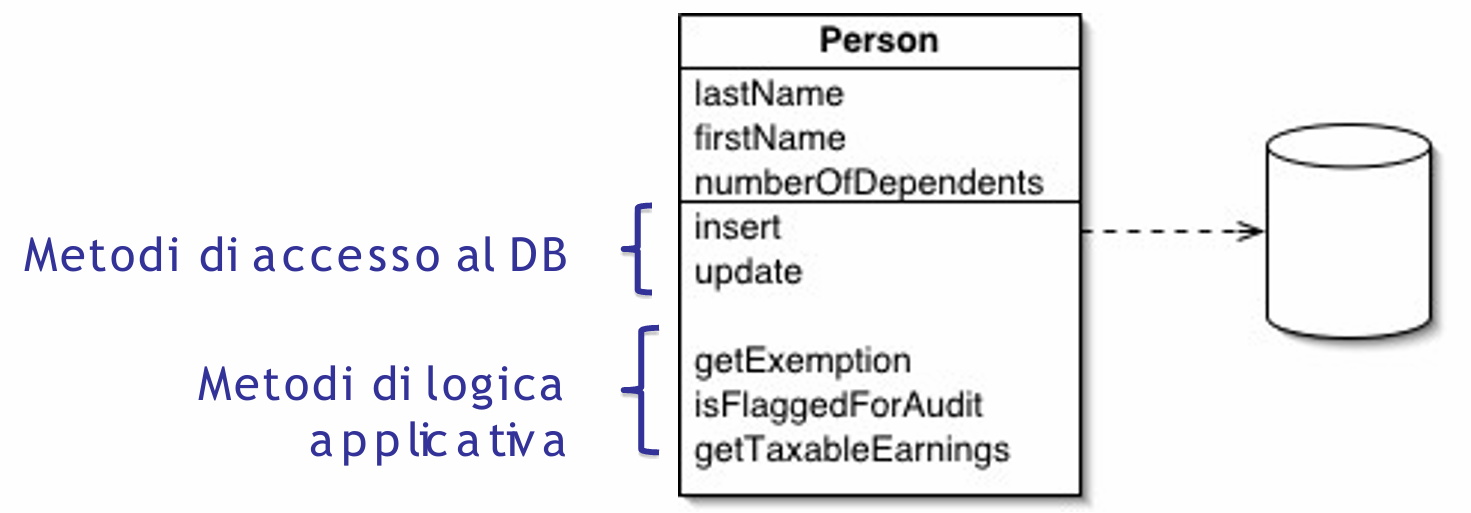
\includegraphics[scale=0.25]{Esercitazione - Design Patterns/Active Record.png}
    \end{center}

    Active Record fa uso di alcuni metodi e strutture dati:
    \begin{enumerate}
        \renewcommand{\labelenumii}{\arabic{enumi}.\arabic{enumii}}
        \item \textbf{Metodo load}: costruisce un'istanza partendo dai risultati generati da una query SQL.
        \item \textbf{Metodi finder} statici: incapsulano le query SQL e ritornano le istanze degli oggetti.
        \item \textbf{Costruttore classico}: costruisce nuove istanze da inserire successivamente nel DB.
        \item \textbf{Metodi di aggiornamento del DB}:
              \begin{enumerate}
                  \item \textbf{update}: aggiorna un record esistente con i valori degli attributi.
                  \item \textbf{insert}: aggiunge un record utilizzando i valori degli attributi.
                  \item \textbf{delete}: elimina il record corrispondente dell'oggetto corrente.
              \end{enumerate}
        \item \textbf{Metodi accessors}:
              \begin{enumerate}
                  \item I metodi \textbf{set} e \textbf{get} per accede ai campi.
                  \item Effettuano la conversione dei dati per memorizzare i valori degli attributi in un formato SQL-oriented.
                  \item Possono richiedere un'immediata sincronizzazione del DB.
              \end{enumerate}
        \item \textbf{Metodo di logica di business}
    \end{enumerate}
    \vspace{0.1cm}

    \resizebox{\columnwidth}{!}{%
        \begin{tabular}{l|l|}
            \hline
            \rowcolor[HTML]{32CB00}
            \multicolumn{1}{|c|}{\cellcolor[HTML]{32CB00}\textbf{Vantaggi}} & \multicolumn{1}{c|}{\cellcolor[HTML]{FE0000}\textbf{Svantaggi}}                                                                                     \\ \hline
            \multicolumn{1}{|l|}{Semplice da implementare e usare}          & \begin{tabular}[c]{@{}l@{}}L'accoppiamento fra la logica applicativa e il DB\\ rende difficile il refactoring dei due progetti\end{tabular}         \\ \hline
                                                                            & \begin{tabular}[c]{@{}l@{}}Si cerca di mantenere una corrispondenza stretta (o quasi)\\ fra lo schema del DB e l'entità del modello OO\end{tabular} \\ \cline{2-2}
        \end{tabular}%
    }
}